\section{Versuchsziele}
\begin{figure}[!h]
		\centering
		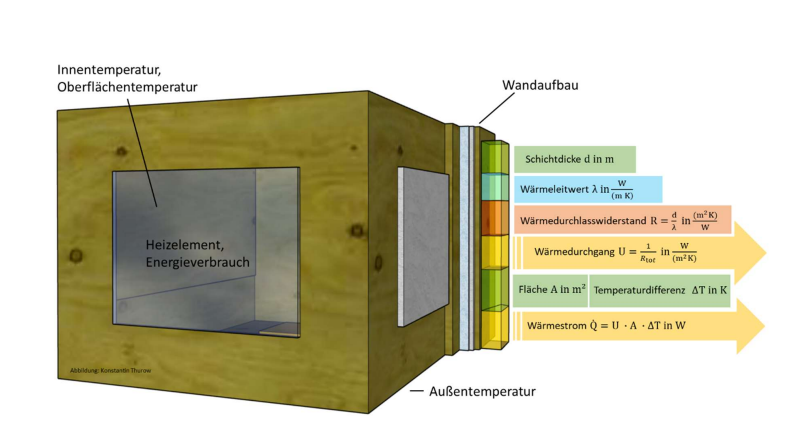
\includegraphics[width=0.7\textwidth]{Abbildungen/Thurow_Deckblatt}
		\caption{Animation des Versuchsaufbaus [Versuchsanleitung] }
		\label{fig:Versuchsaufbau}
\end{figure}

Mit Blick auf die Ziele der Bundesregierung den Endenergieverbrauch bis 2030 um 24\% zu senken gewinnt Energieeffizienz im Bausektor mit rasender Geschwindigkeit an Relevanz. Die Effizienzklassen für Neubauten legen den Fokus auf Dämmungen und können so in den nächsten Jahrzehnten viel Gas und Kohle einsparen. Dieser Versuch soll ein Versändnis für Dämmstoffe und die Klassifikation dieser durch den Wärmedurchgangskoeffizienten (U-Wert) schaffen.  Der Versauchsaufbau besteht aus einem Modellhaus (\autoref{fig:Versuchsaufbau}) austauschbaren Wänden , einem abnehmbaren Dach und einer Glühlampe als Wärmequelle. Ziel ist es aus den aufgenommenen Temperaturdifferenzen in der Auswertung die Wärmeleitfähigkeit und der Wärmedurchgang der einzelnen Materialien zu bestimmen.